\documentclass[11pt,a4paper]{amsart}

\usepackage[margin=1.05in]{geometry}
\usepackage{amsmath,amssymb,amsthm}
\usepackage{graphicx}
\usepackage{booktabs}
\usepackage{array}
\usepackage[colorlinks=true,linkcolor=blue,citecolor=blue,urlcolor=blue]{hyperref}
\usepackage{microtype}

\newtheorem{theorem}{Theorem}[section]
\newtheorem{proposition}[theorem]{Proposition}
\newtheorem{lemma}[theorem]{Lemma}
\newtheorem{corollary}[theorem]{Corollary}
\theoremstyle{definition}
\newtheorem{definition}[theorem]{Definition}
\newtheorem{problem}[theorem]{Open Problem}
\theoremstyle{remark}
\newtheorem{remark}[theorem]{Remark}

\newcommand{\RP}{\mathbb{RP}^2}
\newcommand{\R}{\mathbb{R}}
\newcommand{\Q}{\mathbb{Q}}
\newcommand{\Z}{\mathbb{Z}}

\title[New constructions of four-point orchards]{New constructions of four-point orchards}

\author{Dmitry Kamenetsky}

\date{\today}

\subjclass[2020]{Primary 52C10; Secondary 52C30, 05B30, 51A20}
\keywords{orchard problem, ordinary lines, Melchior's inequality, line arrangements,
celestial configurations, point--line configurations, cross-ratio}

\begin{document}

\begin{abstract}
The orchard problem asks for the maximum number of lines containing exactly $k$ of $n$
points in the real plane. Our main result is a \emph{second-order} application of
Melchior's inequality: rather than applying it to the dual of the point set, we apply
it to the arrangement formed by the rich lines themselves. This yields the new
necessary condition
\[
\sum_{p\in S} w(r_p)\ \le\ \binom{L}{2}-3,
\qquad w(0{,}1{,}2)=0,\ w(3)=3,\ w(j)=\tbinom{j}{2}+j-3\ (j\ge4),
\]
where $L$ is the number of lines carrying at least $k$ points and $r_p$ counts the rich
lines through $p$. Combined with a majorisation argument this gives a closed-form
feasibility test which is strictly stronger than the classical Melchior bound for
small $n$, for every $k\ge4$.

For $k=4$ it yields the exact values $t_4(n)$ at $n=8,9,10,11,13$ by a few lines of
arithmetic, where previously only exhaustive computer searches were available; an
elementary proof of $t_4(12)\le8$, replacing a classification of pseudoline
arrangements; and improvements at $n=14,15$. The inequality is sharp: the optimal
$13$-point configuration attains equality. Writing $T_4$ for the ``at least four''
variant, we obtain $T_4(n)=t_4(n)$ at $n=8,9,10,11,13$.

On the constructive side we exhibit six new lower bounds for the no-five-collinear
variant at $n=28,36,37,40,48,49$, from four-ring \emph{celestial} configurations whose
radii lie in real number fields of degree $6$ and $8$. Finally we verify
$T_4(60)\ge133$ and show that the asymptotic constant $1/28$ is optimal within a
natural family of four-axis constructions. All certificates and verification code are
public, and are available at \url{https://github.com/dimkadimon/Orchard}.
\end{abstract}

\maketitle

\section{Introduction}

The classical orchard-planting problem asks how to place $n$ trees so as to maximise
the number of straight rows containing exactly $k$ trees. For $k=3$ the problem was
essentially settled by Green and Tao \cite{GreenTao2013}, who proved that the maximum
is $\lfloor n(n-3)/6\rfloor+1$ for all sufficiently large $n$. For $k=4$ the situation
is much less complete: the best general upper bound is of order $n^2/14$, the best
constructions give roughly $n^2/28$, and exact values are known only for $n\le20$
\cite{BGS1974,Du2019,OEISA006065}, all but the smallest cases by computer search.

We separate three quantities that are often conflated.

\begin{definition}\label{def:variants}
Let $n\ge k\ge4$. For a finite $S\subset\R^2$ with $|S|=n$, let $t_j(S)$ be the number
of lines containing exactly $j$ points of $S$. Define
\begin{align*}
t_k(n) &= \max_{|S|=n} t_k(S), \\
t_k^{(k+1)}(n) &= \max\{\, t_k(S) : |S|=n,\ t_j(S)=0 \text{ for all } j\ge k+1 \,\}, \\
T_k(n) &= \max_{|S|=n} \#\{\text{lines } \ell : |\ell\cap S|\ge k\}
       = \max_{|S|=n} \sum_{j\ge k} t_j(S).
\end{align*}
\end{definition}

Thus $t_k^{(k+1)}(n)\le t_k(n)\le T_k(n)$. The quantity $t_4^{(5)}$ is the one used by
the online orchard competitions \cite{Contest}, where a row of five or more trees
invalidates an entry; $T_4$ is the natural ``at least four'' variant. The distinction
matters: constructions with long rows are excellent for $T_4$ but inadmissible for
$t_4^{(5)}$.

\subsection*{Contributions}

\begin{enumerate}
\item \textbf{A second-order Melchior bound} (Theorem~\ref{thm:secondorder}), valid for
every $k\ge4$, obtained by applying Melchior's inequality to the arrangement of rich
lines rather than to the dual of the point set.
\item \textbf{New exact values by hand} (Corollary~\ref{cor:exact}):
$t_4(8)=2$, $t_4(9)=3$, $t_4(10)=5$, $t_4(11)=6$, $t_4(13)=9$, together with
$t_4(12)\le8$, $t_4(14)\le11$, $t_4(15)\le13$. The same values hold for $T_4$ at
$n=8,9,10,11,13$.
\item \textbf{Six new algebraic lower bounds} for $t_4^{(5)}$ at $n=28,36,37,40,48,49$
(Section~\ref{sec:constructions}), with exact coordinates, defining polynomials and
diagrams.
\item \textbf{Progress on $T_4$}: $T_4(60)\ge133$, and an optimality result for the
four-axis family (Section~\ref{sec:atleast4}).
\end{enumerate}

We emphasise what is \emph{not} claimed. The general bound
$t_4(n)\le\lfloor(n(n-1)-6)/14\rfloor$ is classical and is stated, for example, in
\cite{MathWorld}. The four-ring sets we use have the shape of the known
\emph{celestial} $(n_4)$ configurations \cite{BermanEtAl,GrunbaumBook}. Our contribution
is the specific parameter choices and record counts, and the new upper-bound argument.

\section{Prior work}\label{sec:prior}

\paragraph{Sylvester--Gallai and Melchior.}
Sylvester's question about ordinary lines was resolved by Gallai \cite{Gallai1944}.
Melchior \cite{Melchior1941} proved the stronger inequality
$t_2\ge3+\sum_{j\ge4}(j-3)t_j$ for the dual arrangement, the engine behind essentially
all upper bounds in this area. Kelly and Rottenberg \cite{KellyRottenberg} extended
$t_2\ge1$ to pseudolines; Bokowski and Pokora \cite{BokowskiPokora} extended the full
Melchior inequality to pseudoline arrangements and derived non-realizability results
that we recover elementarily below. Pokora \cite{Pokora} surveys Hirzebruch-type
inequalities, which give stronger bounds for some $k\ge5$ but, as we check, not for
$k=4$.

\paragraph{The orchard problem.}
Burr, Gr\"unbaum and Sloane \cite{BGS1974} gave the systematic treatment with
constructions and bounds for small $n$; their tables remain the basis of the $n\le25$
data reproduced by Friedman \cite{Friedman} and MathWorld \cite{MathWorld}. Goodman
\cite{Goodman1980} proved a conjecture of \cite{BGS1974}, and F\"uredi and Pal\'asti
\cite{FurediPalasti} gave arrangements with many triple points. Green and Tao
\cite{GreenTao2013} settled the Dirac--Motzkin conjecture and the $k=3$ orchard problem
for large $n$ via a structure theorem for sets with few ordinary lines.

\paragraph{Four-point rows.}
Exact values of $t_4(n)$ for $n\le20$ are recorded in OEIS A006065 \cite{OEISA006065};
$n=19,20$ were established by computer search by Du \cite{Du2019}. Integer-coordinate
records for $n\le60$ are maintained in A172992 \cite{OEISA172992}. Pegg \cite{Pegg2018}
described algebraic-number-field incidence patterns and ``orchard polynomials'';
MathWorld \cite{MathWorld} records five $19$-point patterns with cross-ratio fields
$\Q(\sqrt5)$ and $\Q(\rho)$, $\rho$ the plastic number, and the deletion bound
$t_4(21)\le28$. Elkies \cite{Elkies} constructed sets with many $k$-rich lines in the
regime where the number of points is quadratic in the multiplicity, and formulated the
conjecture $t_k^{(k+1)}(n)=o(n^2)$, open for every $k\ge4$. Solymosi and Stojakovi\'c
\cite{SolymosiStojakovic} proved $t_k^{(k+1)}(n)>n^{2-c/\sqrt{\log n}}$, so no polynomial
saving is possible and the gap between $n^2/28$ and $n^2/14$ is a question about
constants.

\paragraph{Configurations.}
A \emph{celestial} $(n_4)$ configuration is a balanced point--line configuration built
from concentric regular polygons. Berman, G\'evay, Richter-Gebert and Tabachnikov
\cite{BermanEtAl} showed that all \emph{trivial} celestial $(n_4)$ configurations move
in a one-parameter family via the Poncelet porism. These are configurations in the
strict sense (every line has four points \emph{and} every point lies on four lines);
the orchard problem is different, since we count all $4$-point lines and require no
balance. Our four-ring sets are celestial in shape but used as orchards.

\section{Upper bounds}\label{sec:upper}

Throughout, $S\subset\RP$ is a set of $n$ points, $t_j=t_j(S)$, and for a fixed $k\ge4$
we call a line \emph{rich} if it carries at least $k$ points of $S$; $L=\sum_{j\ge k}t_j$
is the number of rich lines. We use
\begin{equation}\label{eq:pairs}
\sum_{j\ge2}\binom{j}{2}t_j=\binom{n}{2},
\end{equation}
and, when the points are not all collinear, Melchior's inequality
\begin{equation}\label{eq:melchior}
t_2\ \ge\ 3+\sum_{j\ge4}(j-3)\,t_j .
\end{equation}
Note that the threshold in \eqref{eq:melchior} is $4$ regardless of $k$; this is why a
single weight function will serve all $k$.

\subsection{The classical bound and its exact slack}

\begin{proposition}[\cite{Melchior1941,MathWorld}]\label{prop:classical}
For $n\ge k+1$,
\[
t_k^{(k+1)}(n)\ \le\ t_k(n)\ \le\ T_k(n)\ \le\
\left\lfloor\frac{\binom{n}{2}-3}{\binom{k}{2}+k-3}\right\rfloor .
\]
For $k=4$ the denominator is $7$, giving $\lfloor(n(n-1)-6)/14\rfloor$.
\end{proposition}

\begin{proof}
If all points are collinear then $T_k=1$ and the bound is trivial. Otherwise
\eqref{eq:pairs} and \eqref{eq:melchior} give
\[
\binom{n}{2}\ \ge\ t_2+\sum_{j\ge k}\binom{j}{2}t_j
\ \ge\ 3+\sum_{j\ge k}\left[\binom{j}{2}+j-3\right]t_j ,
\]
and the bracket is increasing in $j$, so it is at least $\binom{k}{2}+k-3$.
\end{proof}

The proof is an identity, and recording the slack is useful. Let
$F=\sum_{i\ge3}(i-3)f_i\ge0$ be the Melchior face term, where $f_i$ counts the regions
of the dual arrangement with $i$ sides.

\begin{proposition}[slack identity]\label{prop:slack}
If $S$ is not collinear then, for $k=4$,
\[
\binom{n}{2}-3 \;=\; 7L+3t_3+F+\sum_{j\ge5}\left[\binom{j}{2}+j-10\right]t_j ,
\]
where the bracket takes the values $5,11,18,\dots$ at $j=5,6,7,\dots$
\end{proposition}

\begin{proof}
Melchior's proof gives $t_2=3+\sum_{j\ge4}(j-3)t_j+F$. Substituting into
\eqref{eq:pairs} and using $L=t_4+\sum_{j\ge5}t_j$, the coefficient of $t_j$ for
$j\ge5$ is $\binom{j}{2}+(j-3)-7=\binom{j}{2}+j-10$.
\end{proof}

Thus every triple line, every non-triangular region, and every line of five or more
points strictly reduces $L$ below the ceiling of Proposition~\ref{prop:classical}.

\subsection{A second-order Melchior inequality}

The key observation is that Melchior's inequality can be applied a second time, to the
arrangement consisting of the rich lines only. This is a different arrangement from the
dual of $S$, and it sees information that \eqref{eq:melchior} does not.

\begin{definition}
For $p\in S$ let $r_p$ be the number of rich lines through $p$. Define
\[
w(j)=
\begin{cases}
0, & j\le 2,\\
3, & j=3,\\
\dbinom{j}{2}+j-3, & j\ge4 ,
\end{cases}
\]
so that $w(0),w(1),w(2),\dots=0,0,0,3,7,12,18,25,\dots$
\end{definition}

\begin{theorem}[second-order Melchior bound]\label{thm:secondorder}
Let $k\ge4$, let $S\subset\RP$ be finite, and let $\ell_1,\dots,\ell_L$ be $L\ge3$
distinct rich lines of $S$ that are \emph{not} all concurrent. Then
\[
\sum_{p\in S} w(r_p)\ \le\ \binom{L}{2}-3 .
\]
\end{theorem}

\begin{proof}
Let $\mathcal{A}=\{\ell_1,\dots,\ell_L\}$, an essential arrangement of $L\ge3$ lines,
and let $V$ be its vertex set. Split $V=V_S\sqcup V_0$ with $V_S=V\cap S$. A point
$p\in S$ lies in $V_S$ exactly when $r_p\ge2$, and its multiplicity in $\mathcal{A}$ is
then $r_p$. Put
\[
s_j=\#\{p\in S: r_p=j\},\qquad
e_j=\#\{v\in V_0:\ \text{exactly $j$ lines of $\mathcal{A}$ pass through } v\}.
\]
Counting pairs of lines of $\mathcal{A}$ by their intersection point,
\begin{equation}\label{eq:Apairs}
\sum_{j\ge2}\binom{j}{2}(s_j+e_j)=\binom{L}{2}.
\end{equation}
Let $D=\sum_{j\ge2}\binom{j}{2}e_j=\binom{L}{2}-\sum_{p\in S}\binom{r_p}{2}$, so $D\ge e_2$.
Melchior's inequality \eqref{eq:melchior} applied to $\mathcal{A}$ gives
\[
s_2+e_2\ \ge\ 3+\sum_{j\ge4}(j-3)(s_j+e_j)\ \ge\ 3+\sum_{j\ge4}(j-3)s_j .
\]
Since $e_2\le D$,
\[
s_2+\binom{L}{2}-\sum_{p\in S}\binom{r_p}{2}\ \ge\ 3+\sum_{j\ge4}(j-3)s_j ,
\]
and rearranging,
\[
\sum_{p\in S}\binom{r_p}{2}-s_2+\sum_{j\ge4}(j-3)s_j\ \le\ \binom{L}{2}-3 .
\]
The left-hand side is exactly $\sum_p w(r_p)$: terms with $r_p\le1$ vanish, the
$\binom{2}{2}=1$ terms cancel against $-s_2$, terms with $r_p=3$ contribute $3$ each,
and those with $r_p\ge4$ contribute $\binom{r_p}{2}+r_p-3$.
\end{proof}

\begin{remark}
Theorem~\ref{thm:secondorder} requires no hypothesis forbidding long lines, so it
bounds $T_k$ and not merely $t_k^{(k+1)}$. It was checked against $100$ four-point
configurations (the $50$ integer records and our $50$ algebraic entries) and against
$158$ further tests on grids, pencils and random sets for $k=4,\dots,8$; none violates
it, and the optimal $13$-point configuration attains equality.
\end{remark}

\subsection{A closed-form test and new exact values}

Two elementary constraints make Theorem~\ref{thm:secondorder} effective. The rich lines
through $p$ meet only at $p$ and each carries at least $k-1$ further points of $S$, so
\begin{equation}\label{eq:cap}
r_p\le R:=\left\lfloor\frac{n-1}{k-1}\right\rfloor,
\qquad \sum_{p\in S} r_p=\sum_{j\ge k} j\,t_j\ \ge\ kL .
\end{equation}
Also two rich lines meet at most once, so
\begin{equation}\label{eq:convex}
\sum_{p\in S}\binom{r_p}{2}\ \le\ \binom{L}{2}.
\end{equation}

\begin{lemma}[balanced sequences]\label{lem:balanced}
Let $f:\Z_{\ge0}\to\R$ be convex and non-decreasing and fix $n$ and $M\le nR$. Among all
$(r_1,\dots,r_n)\in\{0,\dots,R\}^n$ with $\sum r_i\ge M$, the sum $\sum_i f(r_i)$ is
minimised by the balanced sequence with $\sum r_i=M$: writing $M=qn+\rho$ with
$0\le\rho<n$, it has $n-\rho$ entries $q$ and $\rho$ entries $q+1$.
\end{lemma}

\begin{proof}
For a fixed sum, the balanced vector is majorised by every other vector with that sum,
hence minimises the Schur-convex function $\sum f(r_i)$. As $f$ is non-decreasing, the
minimum over $\sum r_i\ge M$ occurs at $\sum r_i=M$.
\end{proof}

Both $j\mapsto\binom{j}{2}$ and $j\mapsto w(j)$ are convex and non-decreasing (the
successive differences of $w$ are $0,0,3,4,5,6,7,\dots$), so
Lemma~\ref{lem:balanced} applies to \eqref{eq:convex} and to
Theorem~\ref{thm:secondorder} simultaneously. This gives an exact test.

\begin{corollary}\label{cor:test}
Let $k\ge4$, $n\ge k+1$ and $L\ge3$ with $n<(k-1)L+1$. Write $kL=qn+\rho$,
$0\le\rho<n$, and set
\[
\Sigma_2=(n-\rho)\binom{q}{2}+\rho\binom{q+1}{2},\qquad
\Sigma_w=(n-\rho)w(q)+\rho\,w(q+1).
\]
If any of
\[
q+[\rho>0]>R,\qquad \Sigma_2>\binom{L}{2},\qquad \Sigma_w>\binom{L}{2}-3
\]
holds, then no set of $n$ real points has $L$ rich lines. Hence $T_k(n)$ is at most the
largest $L$ passing all three tests.
\end{corollary}

\begin{proof}
If all $L$ rich lines were concurrent at $p$ then $n\ge1+(k-1)L$, excluded by
hypothesis, so Theorem~\ref{thm:secondorder} applies. By \eqref{eq:cap} and
Lemma~\ref{lem:balanced}, $\sum_p\binom{r_p}{2}\ge\Sigma_2$ and
$\sum_p w(r_p)\ge\Sigma_w$, so the three listed inequalities contradict
\eqref{eq:cap}, \eqref{eq:convex} and Theorem~\ref{thm:secondorder} respectively.
\end{proof}

\begin{corollary}[new exact values and improvements]\label{cor:exact}
For $k=4$,
\[
t_4(8)=2,\quad t_4(9)=3,\quad t_4(10)=5,\quad t_4(11)=6,\quad t_4(13)=9,
\]
and
\[
t_4(12)\le8,\qquad t_4(14)\le11,\qquad t_4(15)\le13 .
\]
The same five equalities hold for $T_4$ and for $t_4^{(5)}$. Previously these values
were available only from exhaustive computer search \cite{BGS1974,OEISA006065}.
\end{corollary}

\begin{proof}
We give the two decisive cases; the others are identical arithmetic, and
Table~\ref{tab:bounds} lists them all.

\emph{$n=13$, $L=10$.} Here $4L=40=3\cdot13+1$, so $q=3,\rho=1$ and $R=4$. Then
$\Sigma_w=12\,w(3)+w(4)=36+7=43$, while $\binom{10}{2}-3=42$. As $43>42$, $L=10$ is
impossible. Since $L=9$ is realised with no five collinear, $t_4(13)=T_4(13)=9$.

\emph{$n=12$, $L=9$.} Here $4L=36=3\cdot12$, so $q=3,\rho=0$ and
$\Sigma_w=12\cdot3=36>\binom{9}{2}-3=33$. Hence $T_4(12)\le8$.
\end{proof}

\begin{remark}
The case $T_4(12)\le8$ is equivalent to the non-existence of an arrangement of $12$
pseudolines with $9$ quadruple and $12$ double points, proved by Bokowski and Pokora
\cite[Cor.~1.7]{BokowskiPokora} via an exhaustive sweeping argument; that arrangement is
the dual of the Hesse configuration. Corollary~\ref{cor:exact} replaces the
classification with two lines of counting. We do not know whether $T_4(12)$ is $7$ or
$8$; a hill-climbing search over integer coordinates found nothing beyond $7$.
\end{remark}

\begin{table}[ht]
\centering
\begin{tabular}{rrrrr}
\toprule
$n$ & Prop.~\ref{prop:classical} & Cor.~\ref{cor:test} & exact $t_4(n)$ & best lower bd \\
\midrule
8 & 3 & \textbf{2} & 2 & 2 \\
9 & 4 & \textbf{3} & 3 & 3 \\
10 & 6 & \textbf{5} & 5 & 5 \\
11 & 7 & \textbf{6} & 6 & 6 \\
12 & 9 & 8$^*$ & 7 & 7 \\
13 & 10 & \textbf{9} & 9 & 9 \\
14 & 12 & 11$^*$ & 10 & 10 \\
15 & 14 & 13$^*$ & 12 & 12 \\
16 & 16 & 16 & 15 & 15 \\
17 & 19 & 19 & 16 & 16 \\
18 & 21 & 21 & 18 & 18 \\
19 & 24 & 24 & 20 & 20 \\
20 & 26 & 26 & 23 & 23 \\
21 & 29 & 29 & -- & 24 \\
22 & 32 & 32 & -- & 28 \\
23 & 35 & 35 & -- & 28 \\
24 & 39 & 39 & -- & 31 \\
25 & 42 & 42 & -- & 32 \\
\bottomrule
\end{tabular}
\caption{Upper bounds for $T_4(n)$, hence for $t_4(n)$ and $t_4^{(5)}(n)$. Bold entries
in column 3 are new exact values, where the bound meets the known optimum of
\cite{OEISA006065}; $^*$ marks an improvement over the classical bound that is not yet
matched by a construction. Column 4 is the known exact value for $n\le20$. Column 5 is
the best lower bound for $t_4^{(5)}$ we know: the integer records of
\cite{OEISA172992}, our algebraic entries, and Friedman's table \cite{Friedman}.}
\label{tab:bounds}
\end{table}

The method is not special to $k=4$. Table~\ref{tab:k} records the range over which
Corollary~\ref{cor:test} improves Proposition~\ref{prop:classical} for $k=4,\dots,8$;
the improvements become more substantial as $k$ grows, because the classical bound
weakens faster than the second-order one.

\begin{table}[ht]
\centering
\begin{tabular}{rrrrr}
\toprule
& largest $n$ & \multicolumn{3}{c}{classical $\to$ second-order at} \\
\cmidrule(l){3-5}
$k$ & improved & $n_1$ & $n_2$ & $n_3$ \\
\midrule
4 & 15 & 9$\to$8 & 14$\to$13 & 26$\to$26 \\
5 & 25 & 8$\to$6 & 15$\to$12 & 24$\to$23 \\
6 & 37 & 10$\to$5 & 16$\to$10 & 24$\to$16 \\
7 & 51 & 11$\to$5 & 23$\to$14 & 39$\to$25 \\
8 & 67 & 13$\to$5 & 23$\to$10 & 37$\to$19 \\
\bottomrule
\end{tabular}
\caption{Range of $n\le200$ for which Corollary~\ref{cor:test} improves
Proposition~\ref{prop:classical}, and sample values. For $k=4$ the sample points are
$n=12,15,20$; for $k=5$, $n=15,20,25$; for $k=6$, $n=20,25,30$; for $k=7$, $n=25,35,45$;
for $k=8$, $n=30,40,50$.}
\label{tab:k}
\end{table}

For $k=4$ and $n\ge16$ the three tests never bind, and Proposition~\ref{prop:classical}
remains the best available. Improving the constant $1/14$ asymptotically is open.

\section{Six new algebraic constructions}\label{sec:constructions}

\subsection{Exact arithmetic and the honesty condition}

All constructions are given in a real number field $K=\Q(a)$, where $a$ is a root of a
monic irreducible $p\in\Z[x]$. Each point has coordinates in $K$, written as polynomials
in $a$ of degree $<\deg p$. Collinearity is then decided \emph{exactly} by a determinant
in $K$, never by a floating-point tolerance. A submission consists of $p$ together with
the $n$ coordinate pairs; the count must agree for every real root of $p$, which we
verify.

The competition \cite{Contest} imposes an additional \emph{honesty} condition: the
configuration must not be a projective image of a rational one. Projective maps preserve
cross-ratios, so it suffices to exhibit a $4$-point line with irrational cross-ratio.
For each entry we compute cross-ratios exactly in $K$; the last column of
Table~\ref{tab:records} records how many are irrational.

\subsection{Four-ring celestial sets}

Fix $m\ge5$, radii $r_0=1,r_1,r_2,r_3>0$ and offsets $\varphi_i\in\{0,\pi/m\}$, and put
\begin{equation}\label{eq:celestial}
S(m;\mathbf r,\boldsymbol\varphi)=
\Big\{\, r_i\big(\cos(\tfrac{2\pi j}{m}+\varphi_i),\ \sin(\tfrac{2\pi j}{m}+\varphi_i)\big)
\ :\ 0\le i\le3,\ 0\le j<m \,\Big\},
\end{equation}
a set of $4m$ points on four concentric regular $m$-gons, consecutive rings offset by
half a step. Choosing the $r_i$ so that many transversals meet all four rings produces
$4$-point lines; the required radii are algebraic, and the sets have the celestial shape
familiar from \cite{BermanEtAl,GrunbaumBook}. A \emph{$k4$-ratio} variant allows one
radius to exceed $1$, so the rings need not be nested.

Searching over $(m,\boldsymbol\varphi)$ and solving the collinearity conditions exactly
in the resulting field gave six improvements over the integer records; see
Table~\ref{tab:records} and Figures~\ref{fig:28}--\ref{fig:48}.

Two entries deserve comment. At $n=36$ the configuration has \emph{no} $3$-point lines,
so adjoining any further point of $K$ creates no new $4$-point line; we adjoin
$(a,a)$, giving $37$ points and still $63$ lines, which beats the integer record $62$.
At $n=48$ there are $12$ three-point lines, and the point
\[
\big(1-a-4a^2+4a^3+a^4-a^5,\ \ a+a^3-4a^4+a^6\big)
\]
lies on exactly one of them, giving $49$ points and $97$ lines. We do not picture this
case separately, since it is Figure~\ref{fig:48} together with that single point.

\begin{table}[ht]
\centering
\begin{tabular}{rrrrrlrr}
\toprule
$n$ & $[K:\Q]$ & previous & new & gain & family & $m$ & irr.\ cr. \\
\midrule
28 & 6 & 39 & \textbf{42} & $+3$ & $k4$-ratio & 7 & 42 \\
36 & 6 & 59 & \textbf{63} & $+4$ & celestial & 9 & 63 \\
37 & 6 & 62 & \textbf{63} & $+1$ & celestial$+1$ & 9 & 63 \\
40 & 8 & 69 & \textbf{70} & $+1$ & celestial & 10 & 65 \\
48 & 8 & 93 & \textbf{96} & $+3$ & celestial & 12 & 72 \\
49 & 8 & 96 & \textbf{97} & $+1$ & celestial$+1$ & 12 & 73 \\
\bottomrule
\end{tabular}
\caption{The six new lower bounds for $t_4^{(5)}(n)$. ``Previous'' is the
integer-coordinate record of \cite{OEISA172992}, also the best value we found in the
literature. The defining polynomials are $a^6-7a^4+14a^2-7$ ($n=28$),
$a^6-6a^4+9a^2-3$ ($n=36,37$), $a^8-8a^6+19a^4-12a^2+1$ ($n=40$), and
$a^8-8a^6+20a^4-16a^2+1$ ($n=48,49$). The last column counts $4$-point lines with
irrational cross-ratio, certifying honesty.}
\label{tab:records}
\end{table}

\begin{figure}[ht]
\centering
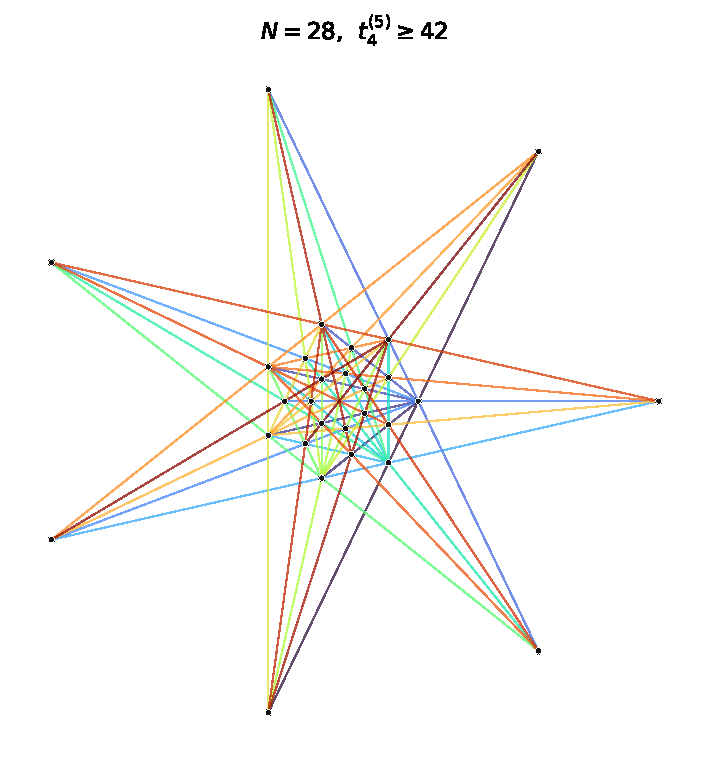
\includegraphics[width=0.60\textwidth]{figures/fig_N28.pdf}
\caption{$n=28$, $42$ four-point lines, no line of five. A $k4$-ratio set with $m=7$;
one radius exceeds $1$, so the outer ring lies far outside the others.
Here $a^6-7a^4+14a^2-7=0$.}
\label{fig:28}
\end{figure}

\begin{figure}[ht]
\centering
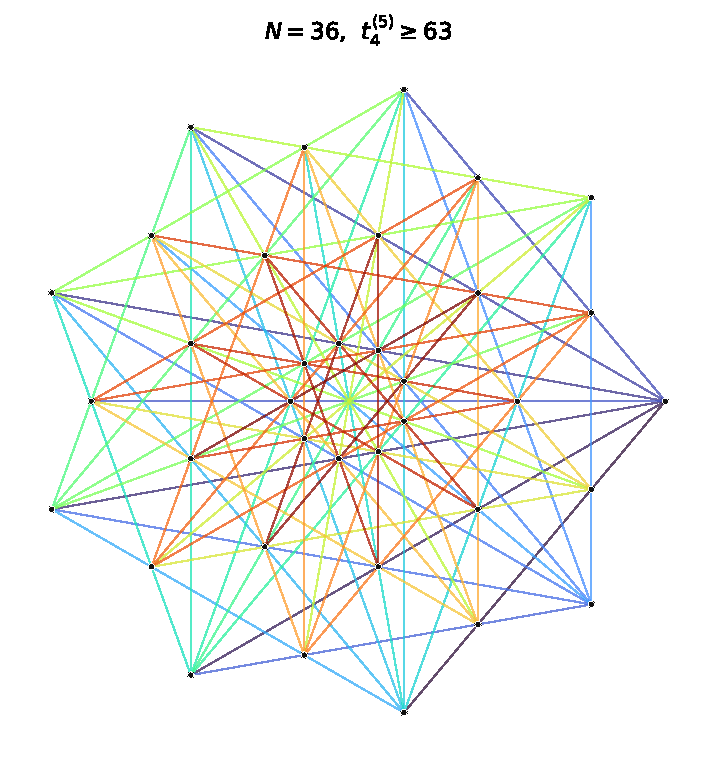
\includegraphics[width=0.60\textwidth]{figures/fig_N36.pdf}
\caption{$n=36$, $63$ four-point lines. Celestial set with $m=9$ and
$a^6-6a^4+9a^2-3=0$. There are no $3$-point lines.}
\label{fig:36}
\end{figure}

\begin{figure}[ht]
\centering
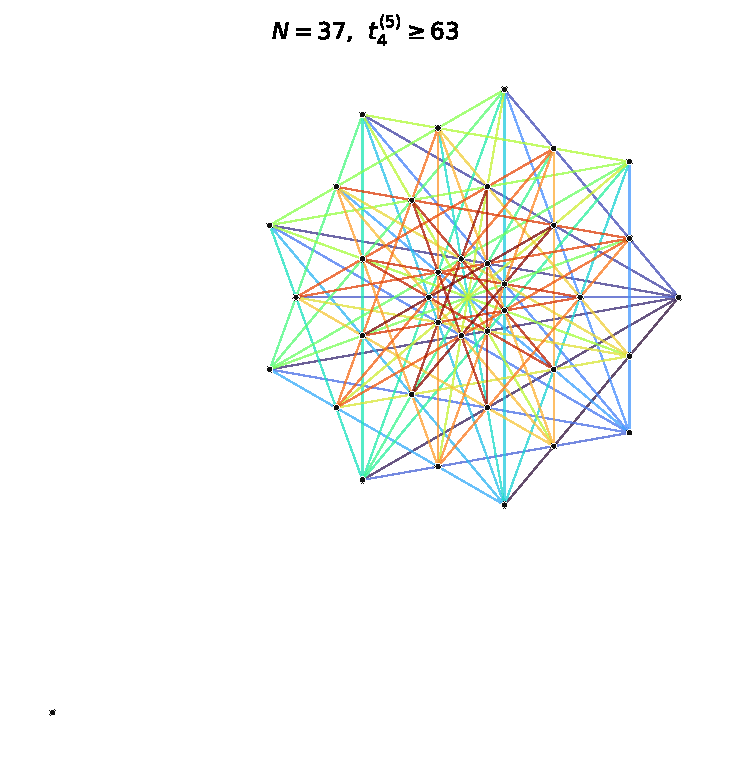
\includegraphics[width=0.60\textwidth]{figures/fig_N37.pdf}
\caption{$n=37$, $63$ four-point lines: Figure~\ref{fig:36} with the point $(a,a)$
adjoined. The count is unchanged, but the integer record at $n=37$ is $62$.}
\label{fig:37}
\end{figure}

\begin{figure}[ht]
\centering
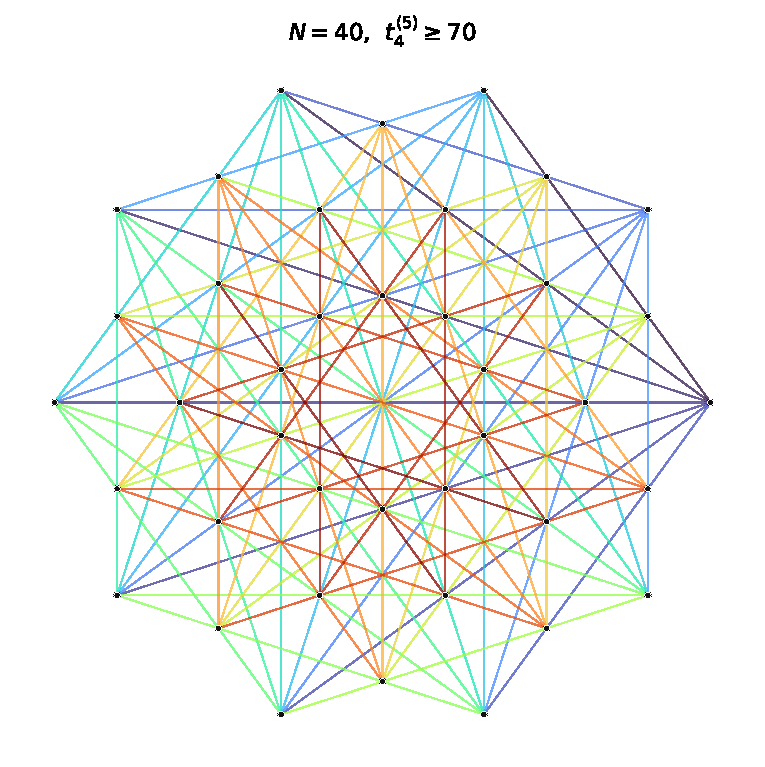
\includegraphics[width=0.60\textwidth]{figures/fig_N40.pdf}
\caption{$n=40$, $70$ four-point lines. Celestial set with $m=10$ in a field of degree
$8$, $a^8-8a^6+19a^4-12a^2+1=0$.}
\label{fig:40}
\end{figure}

\begin{figure}[ht]
\centering
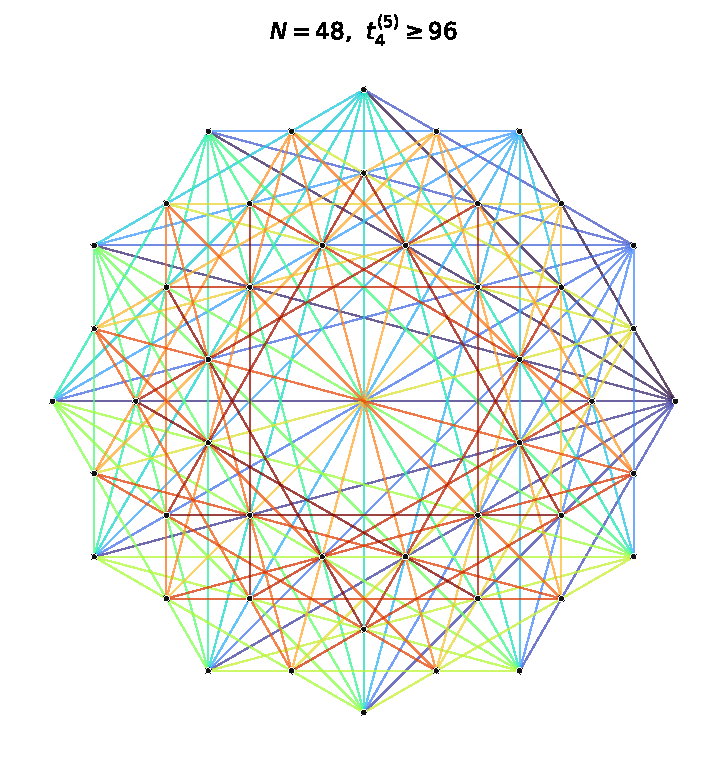
\includegraphics[width=0.60\textwidth]{figures/fig_N48.pdf}
\caption{$n=48$, $96$ four-point lines. Celestial set with $m=12$,
$a^8-8a^6+20a^4-16a^2+1=0$.}
\label{fig:48}
\end{figure}

\subsection{Search and verification}

The search proceeded in three stages. For each $m$ and offset pattern we imposed a set
of desired incidences and solved for the radii symbolically, obtaining a
zero-dimensional ideal whose real solutions give candidate fields. Each candidate was
then scored exactly in $K$. Finally, entries were checked for honesty via cross-ratios
and for root-independence of the count.

We also ran extensive growth and deletion searches: adding a point, deleting a
minimum-degree point, and closing under these operations. Over $164$ algebraic sources
and all $50$ integer records these produced \emph{no} further improvement for
$11\le n\le60$, suggesting the present table is locally optimal for these methods.

\section{The at-least-four variant}\label{sec:atleast4}

\subsection{Four concurrent axes}

Xiang Li \cite{XiangLi} gave the following construction. Place points
\[
\Big(\tfrac{1}{3n+x},0\Big),\quad
\Big(0,\tfrac{1}{n+y}\Big),\quad
\Big(\tfrac{1}{4n+z},\tfrac{1}{4n+z}\Big),\quad
\Big(\tfrac{1}{2n+w},-\tfrac{1}{2n+w}\Big)
\]
for $x\in A$, $y\in B$, $z\in C$, $w\in D$, where $A,B,C,D$ are integer intervals with
$|A|+|B|+|C|+|D|=n$. The line through the first two points is
$(3n+x)X+(n+y)Y=1$; it meets the third axis where the parameter is $x+y$ and the fourth
where it is $x-y$. Hence
\begin{equation}\label{eq:transversal}
\#\{\text{transversals}\}=\#\{(x,y)\in A\times B:\ x+y\in C,\ x-y\in D\},
\end{equation}
which for the balanced choice of intervals is $\lfloor(n^2+12)/28\rfloor$ when
$n\ge28$. All coordinates are rational, so one dilation makes them integral.

The four supporting lines are themselves rich, and in the at-least-four variant they
count:

\begin{proposition}\label{prop:T4family}
For $n\ge28$,
$\displaystyle T_4(n)\ \ge\ \left\lfloor\frac{n^2+12}{28}\right\rfloor+4 .$
\end{proposition}

\begin{proof}
Each axis carries at least four of the points for $n\ge28$, and the transversals of
\eqref{eq:transversal} are distinct from the axes and from one another.
\end{proof}

\subsection{The case $n=60$}

\begin{proposition}\label{prop:T460}
$T_4(60)\ge133$.
\end{proposition}

\begin{proof}
Take $A=B=\{0,\dots,12\}$, $C=\{4,\dots,20\}$, $D=\{-8,\dots,8\}$, i.e.\ denominators
$180+x$, $60+y$, $240+z$, $120+w$. Then \eqref{eq:transversal} counts
$169-10-10-20=129$ pairs. An exact census over $\Q$ of all $\binom{60}{2}$ connecting
lines gives
\[
t_2=400,\quad t_3=56,\quad t_4=129,\quad t_{13}=2,\quad t_{17}=2,
\]
so $T_4=129+4=133$.
\end{proof}

This exceeds the best no-five value at $n=60$ (the integer record $131$). It is
\emph{not} admissible for $t_4^{(5)}$, since two axes carry $17$ points.
Figure~\ref{fig:t4} shows the construction in parameter space. For $n=59$ the family
gives $124+4=128$, tying the integer record; for $n<59$ the no-five records are better.

\begin{figure}[ht]
\centering
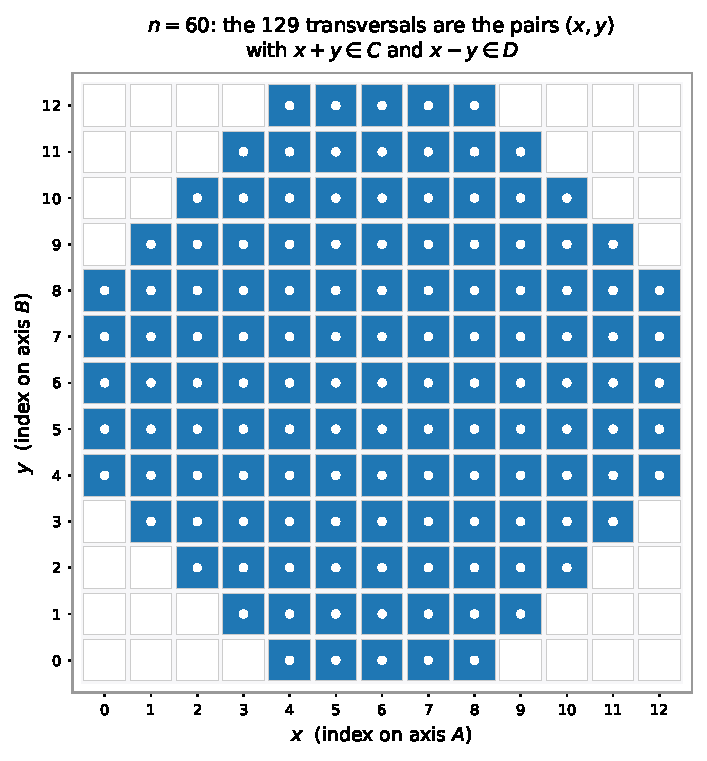
\includegraphics[width=0.58\textwidth]{figures/fig_T4_60.pdf}
\caption{The $129$ transversals of Proposition~\ref{prop:T460} in parameter space. A
cell $(x,y)$ is filled when $x+y\in C=\{4,\dots,20\}$ and $x-y\in D=\{-8,\dots,8\}$; the
two diagonal strips cut the corners of the $13\times13$ box, leaving $129$ cells.
Adding the four axes gives $T_4(60)\ge133$.}
\label{fig:t4}
\end{figure}

\subsection{Optimality within the family}

The construction generalises: replace the axis directions $(1,0),(0,1),(1,1),(1,-1)$ by
$(1,0),(0,1),(p_3,q_3),(p_4,q_4)$. A transversal with parameters $(x,y)$ meets the last
two axes at parameters $p_3x+q_3y$ and $p_4x+q_4y$, so \eqref{eq:transversal} becomes the
number of lattice points in the convex polygon
\[
0\le x\le a,\quad 0\le y\le b,\quad
0\le p_3x+q_3y-o_3\le c,\quad 0\le p_4x+q_4y-o_4\le d,
\]
and the asymptotic constant is its area, maximised subject to $a+b+c+d=1$.

We optimised this over all $231$ pairs of distinct primitive directions with coordinates
in $[-4,4]$. The maximum is $1/28$, attained by the original slopes $(1,1),(1,-1)$ and by
the unimodular choices $(1,1),(1,2)$ and $(1,1),(2,1)$; every other pair gives at most
$1/36$. We also tested whether lattice point sets of other shapes help: disks, squares,
hexagons and triangles all give only about $n^2/67.7$, far below $n^2/28$.

\begin{problem}
Is $T_4(n)=\big(\tfrac1{28}+o(1)\big)n^2$, or can the constant be improved?
Proposition~\ref{prop:classical} gives $1/14$, a factor of two away.
\end{problem}

\section{Reproducibility}

Every count in this paper was obtained by exact arithmetic, either in a number field
$\Q(a)$ or over $\Q$ after clearing denominators; no floating-point tolerance appears in
any certificate. The repository
\begin{center}
\url{https://github.com/dimkadimon/Orchard}
\end{center}
contains the field and scoring libraries, the $50$ algebraic entries, the $60$-point
certificate, the bound computations, the figure scripts, and a verifier that re-derives
every score from the submitted coordinates. Corollary~\ref{cor:test} is implemented in
\texttt{second\_order\_k.py} and was additionally checked against a brute-force
enumeration of \emph{all} admissible degree sequences for $11\le n\le18$, confirming
Lemma~\ref{lem:balanced}.

\section{Open problems}

\begin{problem}
Determine $T_4(12)\in\{7,8\}$, and close the remaining unit gaps at $n=14,15$.
\end{problem}

\begin{problem}
Improve the constant $1/14$ in Proposition~\ref{prop:classical} for $k=4$, or show it is
attained. By \cite{SolymosiStojakovic} no polynomial improvement is possible for
$t_4^{(5)}$, but the constant is wide open.
\end{problem}

\begin{problem}
Does the method extend to a third order, applying Melchior to a still smaller
sub-arrangement? For $k=4$ the three tests of Corollary~\ref{cor:test} stop binding at
$n=16$; a genuinely asymptotic improvement would need a new idea.
\end{problem}

\begin{problem}
Close the gap at $n=24$, where the integer record $31$ still exceeds our best algebraic
entry $29$.
\end{problem}

\section*{Acknowledgements}
The constructions were found by computer search; the exact-arithmetic verifier and all
figures were produced by the code in the accompanying repository. We thank the
maintainers of OEIS A006065 and A172992 and the online orchard competition for making
the record tables public.

\begin{thebibliography}{99}

\bibitem{BermanEtAl}
L.~W. Berman, G.~G\'evay, J.~Richter-Gebert and S.~Tabachnikov,
\emph{Movable $(n_4)$ configurations and the Poncelet porism},
arXiv:2408.09203 (2024); Forum of Mathematics, Sigma (2026).

\bibitem{BokowskiPokora}
J.~Bokowski and P.~Pokora,
\emph{On the Sylvester--Gallai and the orchard problem for pseudoline arrangements},
Period.\ Math.\ Hungar.\ (2018); arXiv:1607.05864.

\bibitem{BGS1974}
S.~A. Burr, B.~Gr\"unbaum and N.~J.~A. Sloane,
\emph{The orchard problem}, Geometriae Dedicata \textbf{2} (1974), 397--424.

\bibitem{Contest}
\emph{Orchard-planting competition}, online record tables for the algebraic and integer
variants, \url{https://www.azspcs.net}.

\bibitem{Du2019}
Z.~H. Du, \emph{Optimal four-point orchards for small $n$}, eMath blog (2019).

\bibitem{Elkies}
N.~D. Elkies, \emph{On some points-and-lines problems and configurations},
arXiv:math/0612749 (2006).

\bibitem{Friedman}
E.~Friedman, \emph{Packing trees in rows},
\url{https://erich-friedman.github.io/packing/trees/}.

\bibitem{FurediPalasti}
Z.~F\"uredi and I.~Pal\'asti,
\emph{Arrangements of lines with a large number of triangles},
Proc.\ Amer.\ Math.\ Soc.\ \textbf{92} (1984), 561--566.

\bibitem{Gallai1944}
T.~Gallai, \emph{Solution to problem 4065},
Amer.\ Math.\ Monthly \textbf{51} (1944), 169--171.

\bibitem{Goodman1980}
J.~E. Goodman, \emph{Proof of a conjecture of Burr, Gr\"unbaum and Sloane},
Discrete Math.\ \textbf{32} (1980), 27--35.

\bibitem{GreenTao2013}
B.~Green and T.~Tao, \emph{On sets defining few ordinary lines},
Discrete Comput.\ Geom.\ \textbf{50} (2013), 409--468.

\bibitem{GrunbaumBook}
B.~Gr\"unbaum, \emph{Configurations of Points and Lines},
Graduate Studies in Mathematics \textbf{103}, Amer.\ Math.\ Soc., 2009.

\bibitem{KellyRottenberg}
L.~M. Kelly and R.~Rottenberg, \emph{Simple points in pseudoline arrangements},
Pacific J.\ Math.\ \textbf{40} (1972), 617--622.

\bibitem{MathWorld}
E.~W. Weisstein, \emph{Orchard-planting problem}, MathWorld,
\url{https://mathworld.wolfram.com/Orchard-PlantingProblem.html} (accessed Nov.\ 2026).

\bibitem{Melchior1941}
E.~Melchior, \emph{\"Uber Vielseite der projektiven Ebene},
Deutsche Math.\ \textbf{5} (1941), 461--475.

\bibitem{OEISA006065}
OEIS Foundation Inc., \emph{Entry A006065: maximal number of four-point lines},
\url{https://oeis.org/A006065}.

\bibitem{OEISA172992}
OEIS Foundation Inc., \emph{Entry A172992: integer four-point orchard records},
\url{https://oeis.org/A172992}.

\bibitem{Pegg2018}
E.~Pegg~Jr., \emph{Orchard planting polynomials}, Wolfram Blog (2018).

\bibitem{Pokora}
P.~Pokora, \emph{Hirzebruch-type inequalities viewed as tools in combinatorics},
Electron.\ J.\ Combin.\ \textbf{28} (2021), \#P1.9; arXiv:1808.09167.

\bibitem{SolymosiStojakovic}
J.~Solymosi and M.~Stojakovi\'c,
\emph{Many collinear $k$-tuples with no $k+1$ collinear points},
Discrete Comput.\ Geom.\ (2013); arXiv:1107.0327.

\bibitem{XiangLi}
X.~Li, \emph{A four-point-line construction for OEIS A172992},
OEIS attachment \texttt{a172992\_1.pdf} (September 2026).

\end{thebibliography}

\end{document}
